%%%%%%%%%%%%%%%%%%%%%%%%%%%%%%%%%%%%%%%%%%%%%%%%%%%%%%%%%%%%%%%%%%%%%%%%%%%%%%%%%%%%%%
% Arithmetick und Datentypen
%%%%%%%%%%%%%%%%%%%%%%%%%%%%%%%%%%%%%%%%%%%%%%%%%%%%%%%%%%%%%%%%%%%%%%%%%%%%%%%%%%%%%%
\section{Arithmetick und Datentypen}

\begin{minipage}{0.4\textwidth}
	\begin{tabular}{l|l}
		\multicolumn{2}{l}{\textbf{Logische Operatoren}}  \\
		\multicolumn{2}{l}{für bit, bit\_vector, std\_(u)logic, std\_(u)logic\_vector }\\
		mit STD Library		& mit ieee.numeric\_std {\tiny ieee.numeric\_bit}\\
		\hline
		$\cdot$ and, nand	& $\cdot$ + ,-\\
		$\cdot$ or, nor		& $\cdot$ signed, unsigned \\
		$\cdot$ xor, xnor	& $\cdot$ abs, mod, rem\\
		$\cdot$ not			& $\cdot$ *, /, **\\
	\end{tabular}
	
	\subsection{Datentypen}
	
	\begin{VHDL}
-- Aufzaelungstyp
type <my_type> is ({my_value_1,} my_value_n);
type traffic_light is (rot, bruen, orange);-- Bsp.
-- Physikalische Typen
tyle PHYS_NAME is range RANGE_OF_VALUES
units
	BASE_UNIT;
	{MULTIPLES;}
end units
tyle CAPACITANCE is range 0 to 1E30 -- Bsp
units
	pF;
	nF = 1000 pF;
	uF = 1000 nF;
end units
-- Arraytyp
type ARRAY_NAME is array
	(UPPER_LIM downto LOWER_LIM) of BASE_TYPE;
type VECTOR_1 is array  -- Bsp
	(9 downto 0) of integer;
	\end{VHDL}
	
\end{minipage}
\begin{minipage}{0.6\textwidth}
	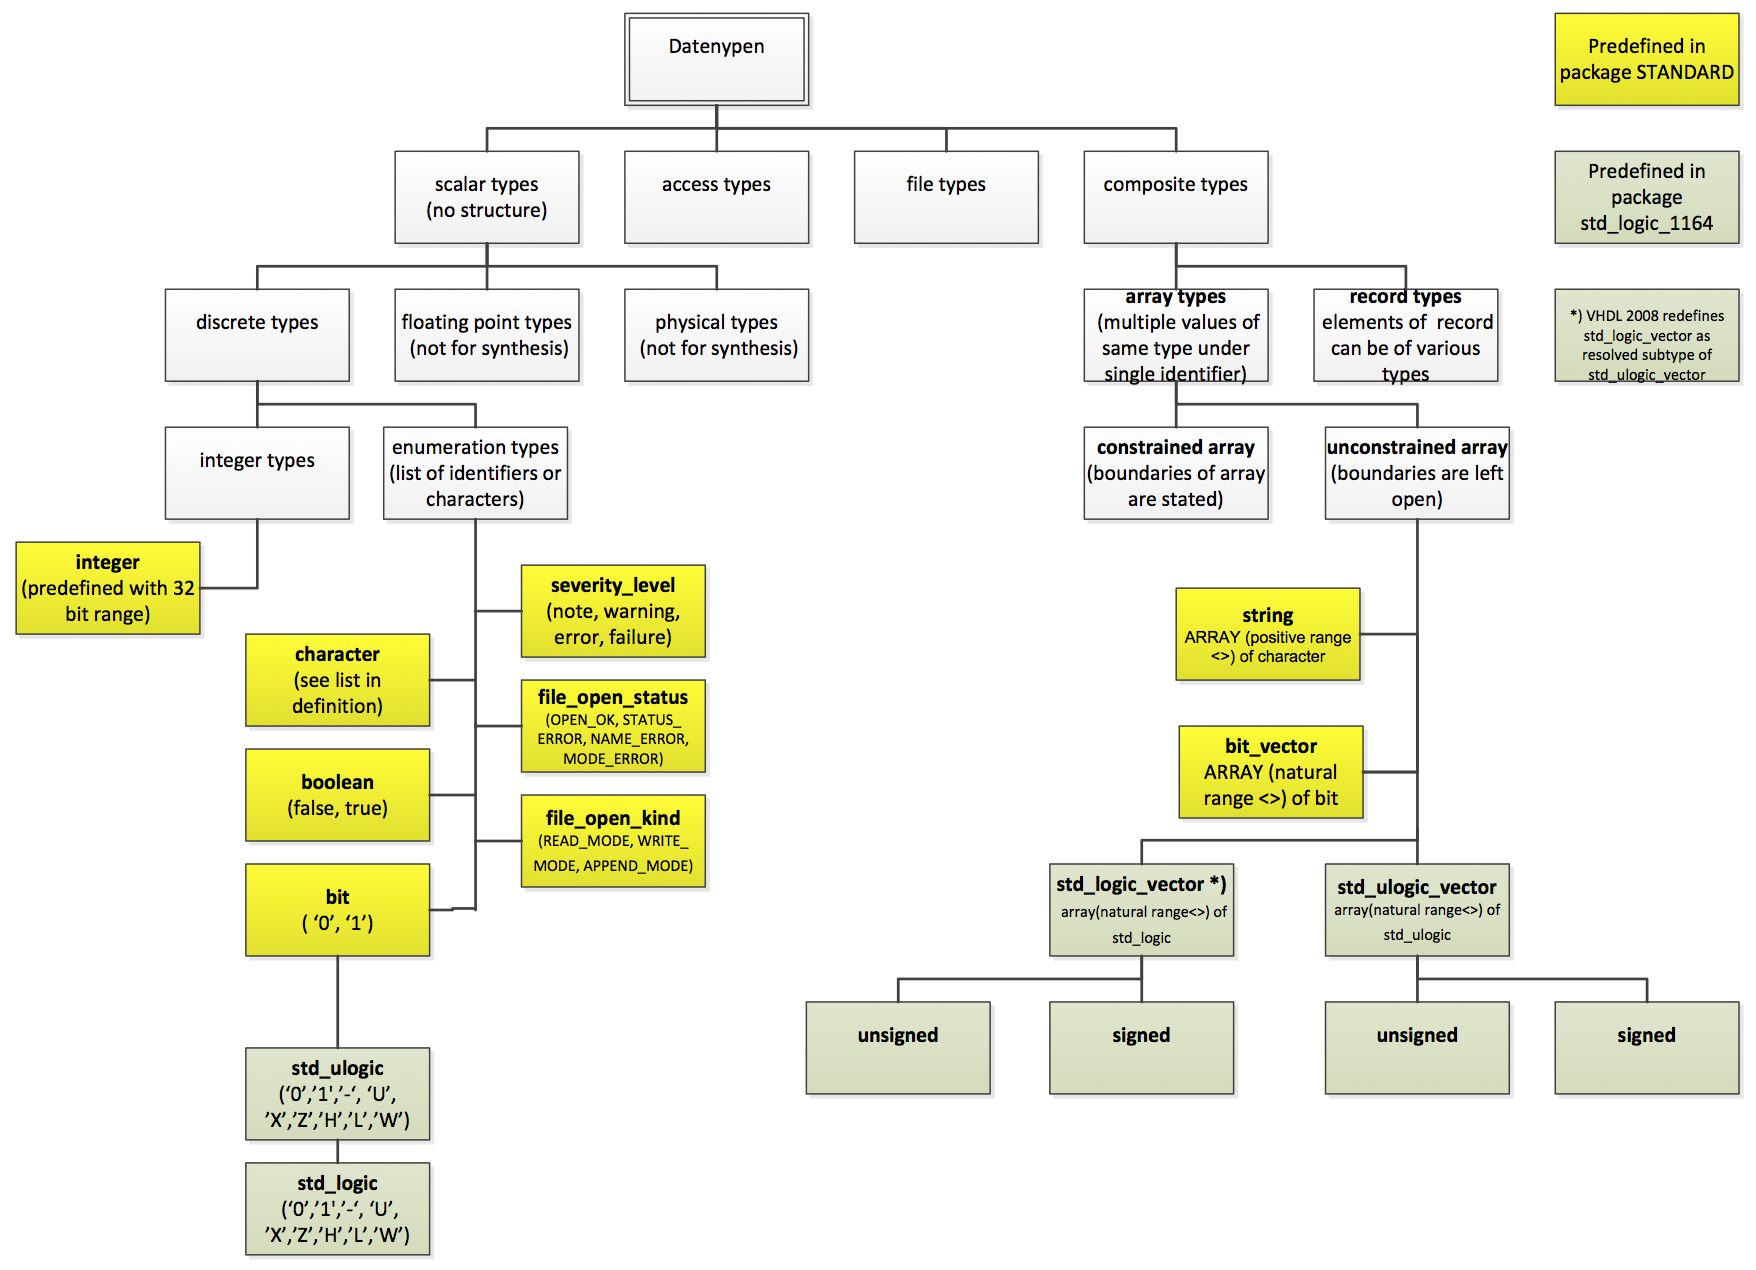
\includegraphics[width=\textwidth]{./bilder/Datentypen}
	
	\begin{minipage}{0.02\textwidth}
		\text{ } %platzhalter
	\end{minipage}
	\begin{minipage}{0.72\textwidth}
		\begin{VHDL}
	-- Resize
	function RESIZE (ARG: signed; NEW_SIZE: natural)
	return signed;
	y <= resize(A,y'length) + resize(B,y'length);
	-- Type_cast
	target_signal <= target_type (source_signal);
	-- Type_convercion
	target_signal <= to_<target_type> (source_signal);	\end{VHDL}	
	\end{minipage}
	\begin{minipage}{0.02\textwidth}
		\text{ } %platzhalter
	\end{minipage}
	\begin{minipage}{0.18\textwidth}
		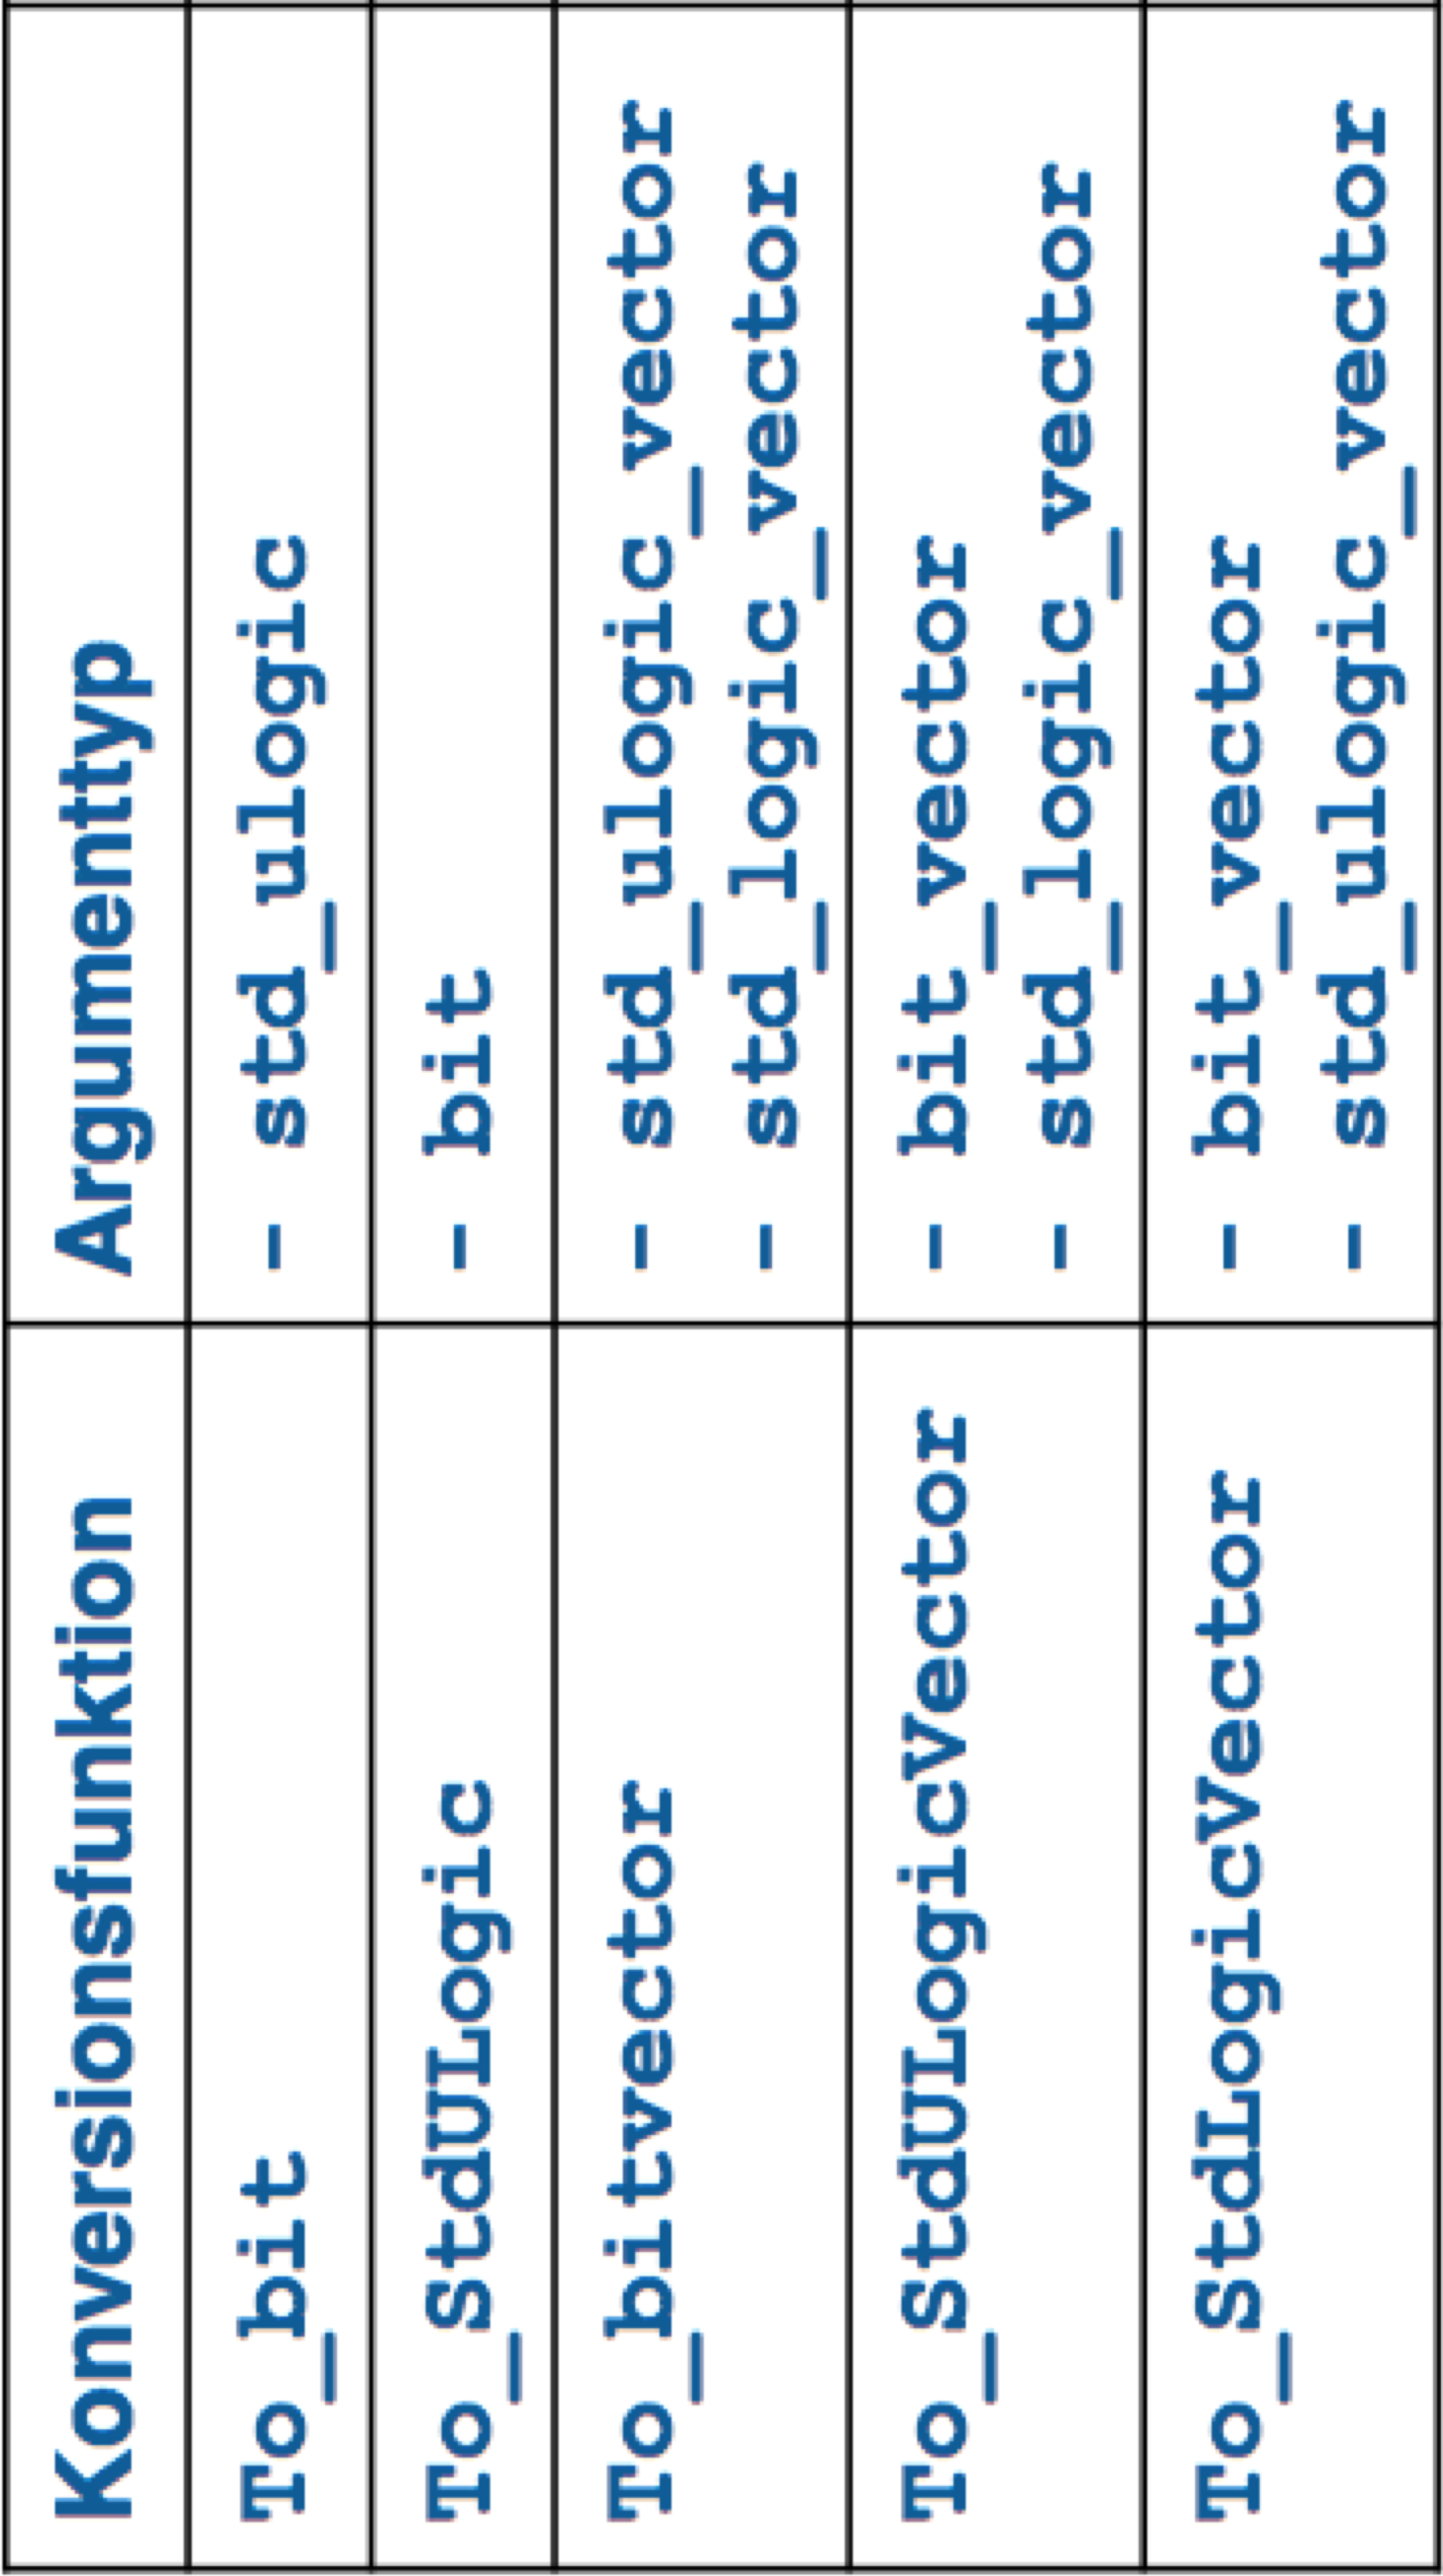
\includegraphics[width=\textwidth]{./bilder/Konversion}
	\end{minipage}
\end{minipage}
